\documentclass[11pt, oneside]{article}   	% use "amsart" instead of "article" for AMSLaTeX format


% \usepackage{draftwatermark}
% \SetWatermarkText{Draft}
% \SetWatermarkScale{5}
% \SetWatermarkLightness {0.9} 
% \SetWatermarkColor[rgb]{0.7,0,0}


\usepackage{geometry}                		% See geometry.pdf to learn the layout options. There are lots.
\geometry{letterpaper}                   		% ... or a4paper or a5paper or ... 
%\geometry{landscape}                		% Activate for for rotated page geometry
%\usepackage[parfill]{parskip}    		% Activate to begin paragraphs with an empty line rather than an indent
\usepackage{graphicx}				% Use pdf, png, jpg, or eps� with pdflatex; use eps in DVI mode
								% TeX will automatically convert eps --> pdf in pdflat						
								% TeX will automatically convert eps --> pdf in pdflatex		
\usepackage{amssymb}
\usepackage{mathrsfs}
\usepackage{hyperref}
\usepackage{url}
\usepackage{subcaption}
\usepackage{authblk}
\usepackage{amsmath}
\usepackage{mathtools}
\usepackage{graphicx}
\usepackage[export]{adjustbox}
\usepackage{fixltx2e}
\usepackage{hyperref}
\usepackage{alltt}
\usepackage{color}
\usepackage[utf8]{inputenc}
\usepackage[english]{babel}
\usepackage{float}
\usepackage{bigints}
\usepackage{braket}
\usepackage{siunitx}



\newcommand{\argmax}{\operatornamewithlimits{argmax}}
\newcommand{\argmin}{\operatornamewithlimits{argmin}}

\title{Notes on the Dual Beam Splitter Experiment}
\author{David Meyer \\ dmm@\{1-4-5.net,uoregon.edu\}}

\date{Last update: April 20, 2016}							% Activate to display a given date or no date



\begin{document}
\maketitle

\section{Introduction}
This document describes an experimental setup that cannot be described in a natural way by classical physics yet still  has a simple quantum explanation \cite{Aharonov:aa, Henault:2015aa}. The implication/point is this that the description of the universe given by quantum mechanics differs in fundamental ways from the classical description. In addition, this quantum description is often at odds with our intuition, which is primarily based on observations of macroscopic phenomena. Not that these observations aren't an extremely good approximation, they are, and what's more they are generally consistent with classical physics. 

\begin{figure}
\center{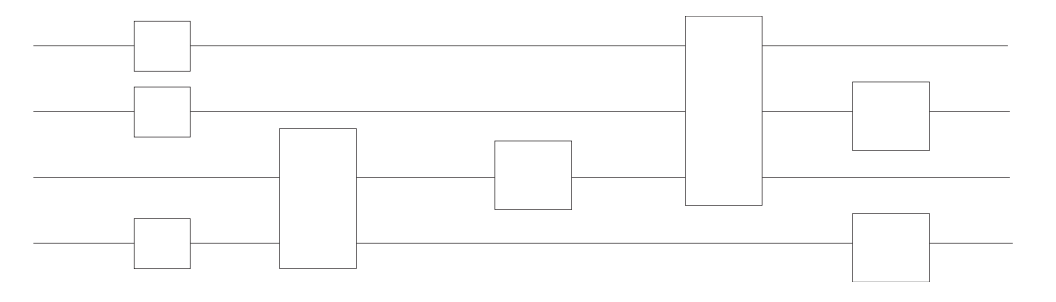
\includegraphics[scale=0.8, frame] {images/circuit}}
\caption{A curcuit of depth 5 and space 4 with 8 gates}
\label{fig:circuit}
\end{figure}


\subsection{Preliminaries: Linear Algebra Formulation of the Circuit Model}

In this section we take a brief look at the circuit model of computation. The model is described in terms of vectors and matrices.  So suppose you are given a description of a circuit like the one shown in Figure \ref{fig:circuit} along with some specification of some input bit values. If you were asked to predict the output of the circuit,  you might trace through the circuit from left to right, updating the values of the bits stored on each of the wires after each gate. In other words, you would follow the \emph{state} of the bits on the wires as they progress through the circuit. For a given point in the circuit then, we can refer to the state of the bits on the wires at that point in the circuit simply as the \emph{state} of the computation at that point. Importantly, the \emph{memory} of the circuit is the state of the wires, and the \emph{gates} are transformations on that state. 

\bigskip
\noindent
Given this model, we can conceptualize the state associated with a given point in a deterministic circuit by listing the values of the bits on each of the wires in the circuit. The \emph{state} of any particular wire at a given point in a circuit, of course, is just the value of the bit on that wire (0 or 1). For a probabilistic circuit, however, this simple description is not enough. In particular, consider a single bit that is in state 0 with probability $p_0$ and in state 1 with probability $p_1$ (where $p_0 + p_1 = 1$). We can represent this state by a  2-dimensional vector of probabilities:
\begin{flalign*}
\begin{pmatrix}
p_0 \\
p_1
\end{pmatrix}
\end{flalign*}

\bigskip
\noindent
Note that this description can also be used for deterministic circuits. A wire in a deterministic circuit whose state is 0 could be specified by the probabilities $p_0 = 1$ and $p_1 = 0$, and the corresponding vector
\begin{flalign*}
\begin{pmatrix}
1\\
0
\end{pmatrix}
\end{flalign*}

\noindent
Similarly, a wire in state 1 could be represented by the probabilities $p_0 = 0$,
$p_1 = 1$, and the vector
\begin{flalign*}
\begin{pmatrix}
0\\
1
\end{pmatrix}
\end{flalign*}

\bigskip
\noindent
Since the standard representation the states of wires (or collections of wires) in a circuit is by vectors, we will also want to represent gates in the circuit by operators that act on these state vectors. Hence these operators are  most conveniently described by matrices. Consider, for example,  the logical NOT gate. We would like to define an operator (matrix) that behaves on state vectors in a manner consistent with the behavior of the NOT gate. If we know a wire is in state 0 (so $p_0 = 1$), the not gate maps it to state 1 (so  $p_1 = 1$), and vice versa. In terms of the vector representations of these states, we have

\begin{flalign*}
\text{NOT} \;
\begin{pmatrix}
0\\
1
\end{pmatrix}
=
\begin{pmatrix}
1\\
0
\end{pmatrix}
\end{flalign*}

\noindent
Similarly, 
\begin{flalign*}
\text{NOT} \;
\begin{pmatrix}
1\\
0
\end{pmatrix}
=
\begin{pmatrix}
0\\
1
\end{pmatrix}
\end{flalign*}

\noindent
The next step is to characterize the \emph{transformation} (gate) as a matrix. In the case of the NOT gate, we have

\begin{flalign*}
\text{NOT} \equiv
\begin{pmatrix}
0 & 1\\
1 & 0
\end{pmatrix}
\end{flalign*}

\noindent
So now if we want to apply the NOT gate to a wire in a given state, we multiply the state vector on the left by the matrix representation of the NOT gate:

\begin{flalign*}
\text{NOT} \;
\begin{pmatrix}
p_0\\
p_1
\end{pmatrix}
=
\begin{pmatrix}
0 & 1\\
1 & 0
\end{pmatrix}
\begin{pmatrix}
p_0\\
p_1
\end{pmatrix}
\end{flalign*}

\bigskip
\noindent
Now we want to describe the state associated with a given point in a probabilistic circuit having two wires.  Let the state of the first wire at the given point be 0 with probability $p_0$ and 1 with probability $p_1$ and the state of the second wire at this point be 0 with probability $q_0$ and 1 with probability $q_1$. The four possibilities for the combined state of both wires at the given point are \{00,01,10,11\}, where the binary string ij indicates that the first wire is in state i and the second wire in state j. Then  the combined state of both wires can be described by the column vector of probabilities:

\begin{flalign*}
\begin{pmatrix}
p_0 q_0\\
p_0 q_1 \\
p_1 q_0 \\
p_1 q_1
\end{pmatrix}
\end{flalign*}

\bigskip
 \noindent
What this is setting up is that the state is really the \emph{tensor product} of the 2-dimensional
vectors for the states of the first and second wires:

\begin{flalign*}
\begin{pmatrix}
p_0 q_0\\
p_0 q_1 \\
p_1 q_0 \\
p_1 q_1
\end{pmatrix}
=
\begin{pmatrix}
p_0\\
p_1
\end{pmatrix}
\otimes
\begin{pmatrix}
q_0\\
q_1
\end{pmatrix}
\end{flalign*}

\subsection{Aside: The Dirac Notation}
The Dirac Notation, also known as bra-ket notation, was invented by Paul Dirac for use in quantum mechanics \cite{2000RPPh...63.1893G}. 
The problem Dirac faced was that, while  column vector notation is ubiquitous in linear algebra,  the standard notation was often cumbersome
 in quantum mechanical derivations. This is especially true when dealing with both inner and outer products (e.g., with multiple qubits).  For
  example, when we define $\psi$  to be a vector it is not clear whether $\psi$  is a row or a column vector. Similarly,  if $\phi$ and $\psi$ 
  are vectors then it is equally unclear if $\phi \psi$ is even 
 defined because the shapes of $\phi$ and $\psi$ may be unclear in the context\footnote{Recall that matrix multiplication is only defined when the 
 number of columns of the first matrix (vector) is equal to the number of rows in the second matrix.}. Beyond the  ambiguity about the shapes of 
 vectors, expressing even simple vectors using the linear algebraic notation introduced earlier can be very less elegant. For example, if we wish to describe an 
n-qubit state where each qubit takes the value 0 then we would express the state as

\begin{flalign*}
\begin{pmatrix}
1 \\
0
\end{pmatrix}
\otimes
\hdots
\otimes
\begin{pmatrix}
1 \\
0
\end{pmatrix}
\end{flalign*}


\bigskip
\noindent
So one of the problems here is that evaluating this tensor product is impractical because the vector lies in an exponentially large space. So maybe this notation is the best description 
of the state that can be given using the previous notation (it is really speculation; I have no idea how one would prove such an assertion). In any event, Dirac's approach was to 
define a new notation that is designed to fit the needs of quantum mechanics. 

\subsubsection{Preliminaries}
In order to confront both the bulky notation of linear algebra (at least when applied to quantum mechanics use cases) and the ambiguity posed by standard vector notation, 
Dirac proposed a new notation for two kinds of vectors frequently used in quantum mechanics:  a "ket" vector, denoted 
$\ket{a}$, and a "bra" vector, which is denoted $\bra{a}$. The naming comes from the fact that when put together they form a "bra[c]ket" or inner product.  So if If $\phi$ is a column vector 
then we can write it in Dirac notation as $\ket{\phi}$, where the $\ket{\cdot}$ denotes that it is a unit column vector, i.e., a ket vector. Similarly, the row vector 
$\psi^\dagger$  is expressed as $bra{\psi}$, where $\psi^\dagger$  is obtained by applying entry-wise complex conjugation to the elements of the transpose of $\psi$ (more on this below). 
The bra-ket notation also implies that $\bra{\psi} \psi \rangle$  is the inner product of vector $\psi$ with itself, which is by definition 1.

\bigskip
\noindent
The ket vector can be represented as a column vector:

\begin{equation*}
\ket{a} = 
\begin{pmatrix}
a_1\\
\vdots \\
a_n
\end{pmatrix}
\end{equation*}

\noindent
where $n$ is typically three or four (representing the dimensionality of space or space-time) and $a_i$ is a complex number, namely $a_i \in \mathbb{C}$.

\bigskip
\noindent
Similarly, a bra vector can be represented as


\begin{equation*}
\bra{a} = \big (a^*_1, a^*_2, \hdots, a^*_n \big )
\end{equation*}

\bigskip
\noindent
where $a^*_i$ is the \emph{complex conjugate} of $a_i$. That is, if $z$ is a complex number, it can be written as $z = x +iy$, where $x,y \in \mathbb{R}$ and  $i = \sqrt{-1}$.
Then the complex conjugate of $z$, denoted $z^*$ where $z^* = x -iy$,  the reflection of $z$ around the real axis. This is depicted in 
Figure \ref{fig:cc} \footnote{Note that $\bar{z} = z^*$ in Figure \ref{fig:cc}.}. 



\begin{figure}
\center{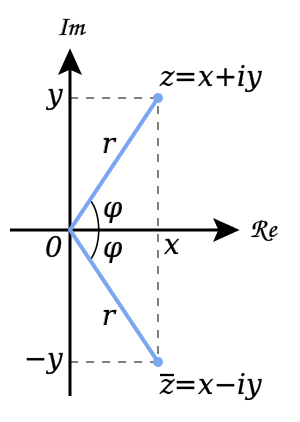
\includegraphics[scale=0.45] {images/complex_congugate.png}}
\caption{Complex conjugates. Image courtesy Wikipedia. }
\label{fig:cc}
\end{figure}


\bigskip
\noindent
The \emph{modulus} of $z$, denoted as $|z|^2$,  is the length of the  directed line segment drawn from the origin of the complex plane to the point $(x, y)$.  
This directed line segment is also the vector that represented by $x + iy$, so the modulus of a complex number is the same thing as the magnitude (or length) 
of the vector representing $z$. As a result $|z|^2 = x^2 +y^2$ by the Pythagorean Theorem. This also means that $|z|^2 = |z^*|^2$.

\bigskip
\noindent
Another interesting property of $z$ is that if you multiply $z$ by its complex conjugate $z^*$ you get
\begin{flalign*}
z z^* 
&= (x + iy) (x - iy) \\
&= x^2 + y^2
\end{flalign*}

\bigskip
\noindent
Note also that the complex conjugate of some $x \in \mathbb{R}$ is simply $x$. That is, for $x \in \mathbb{R}$, $x = x^*$.

\bigskip
\noindent
Now we're ready to do some arithmetic. Consider first that $\ket{a} + \ket{b} = \ket{c}$. Why? We can see 
this (without loss of generality) in three dimensions:

\begin{flalign*}
\begin{pmatrix}
a_1\\
a_2 \\
a_3
\end{pmatrix}
+
\begin{pmatrix}
b_1\\
b_2 \\
b_3
\end{pmatrix}
=
\begin{pmatrix}
a_1 + b_1\\
a_2 + b_2 \\
a_3 + b_3
\end{pmatrix}
\end{flalign*}

\bigskip
\noindent
ket vectors, being column vectors,  follow basic linear algebra properties, such as 

\begin{flalign*}
\alpha \ket{a} = 
\alpha \begin{pmatrix}
a_1\\
a_2 \\
a_3
\end{pmatrix}
=
\begin{pmatrix}
\alpha a_1\\
\alpha a_2 \\
\alpha a_3
\end{pmatrix}
\end{flalign*}

\bigskip
\noindent
Now, what happens if you multiply a bra vector by a ket vector? That is, $\braket{a | b}$? Here the brackets indicate the inner product. 
In our three dimensional example, we get 

\begin{flalign*}
\braket{a | b} =
\big (a^*_1, a^*_2, a^*_3 \big ) 
\begin{pmatrix}
b_1\\
b_2 \\
b_3
\end{pmatrix}
= a^*_1  b_1 + a^*_2 b_2 + a^*_3 b_3
\end{flalign*}

\bigskip
\noindent
Similarly, $\braket{b | a} = b^*_1 a_1 + b^*_2a_2 + b^*_3 a_3$. What about $\braket{b | a}^*$? Well,
$\braket{b | a}^* = b_1 a_1^* + b_2 a_2^* + b_3 a^*_3$. So we see that $\braket{a | b} = \braket{b | a}^*$.


\bigskip
\noindent
Now lets look at operations on a square matrix $M$. Suppose that $M$ is a $3 \times 3$ matrix. Then we can write $M$ 
as the matrix of elements $m_{i,j}$, where $m_{i,j}$  is the element in the $i^\text{th}$ row and
$j^{\text{th}}$ column, as follows

\begin{equation*}
M =
\begin{pmatrix}
m_{11} & m_{12} & m_{13} \\
m_{21} & m_{22} & m_{23} \\
m_{31} & m_{32} & m_{33} \\
\end{pmatrix}
\end{equation*}

\bigskip
\noindent
What about $M^*$? Well this is just

\begin{equation*}
M^* =
\begin{pmatrix}
m_{11}^* & m_{12}^* & m_{13}^* \\
m_{21}^* & m_{22}^* & m_{23}^* \\
m_{31}^* & m_{32}^* & m_{33}^* \\
\end{pmatrix}
\end{equation*}

\bigskip
\noindent
The \emph{transpose} of a matrix $M$, $M^\text{T}$ is defined as

\begin{equation*}
M^\text{T} =
\begin{pmatrix}
m_{11} & m_{21} & m_{31} \\
m_{12} & m_{22} & m_{32} \\
m_{13} & m_{23} & m_{33} \\
\end{pmatrix}
\end{equation*}

\bigskip
\noindent
Essentially the transpose of a matrix is the reflection around the diagonal. Another important matrix, $M^\dagger$, is the combination of the transposition and
the complex conjugate. That is

\begin{equation*}
M^\dagger =
\begin{pmatrix}
m_{11}^* & m_{21}^* & m_{31}^* \\
m_{12}^* & m_{22}^* & m_{32}^* \\
m_{13}^* & m_{23}^* & m_{33}^* \\
\end{pmatrix}
\end{equation*}

\bigskip
\noindent
In the case where $M = M^\dagger$, $M$ is called Hermitian. For a (somewhat contrived) example suppose

\begin{flalign*}
M = \begin{pmatrix}
1 & i + 1 \\
i - 1 & 3
\end{pmatrix}
\end{flalign*}

\bigskip
\noindent
To find $M^\dagger$, we first take the transpose of $M$

\begin{equation*}
M^\text{T} =
\begin{pmatrix}
1 &  i - 1 \\
i + 1 & 3 \\
\end{pmatrix}
\end{equation*}

\bigskip
\noindent
and then take the complex conjugate, resulting in 

\begin{flalign*}
M^\dagger = \begin{pmatrix}
1 & i + 1 \\
i - 1 & 3
\end{pmatrix}
\end{flalign*}

\bigskip
\noindent
or just $M$. So we can see that in this case, $M = M^\dagger$ , that is, $M$ is Hermitian.

\bigskip
\noindent
Next we want to ask what happens if we have a matrix times a ket vector, that is, $M \ket{a}$. An example in two dimensions would
look like
\begin{equation*}
M \ket{a} = \begin{pmatrix}
m_{11} & m_{12}\\
m_{21} & m_{22} 
\end{pmatrix}
\begin{pmatrix}
a_1 \\
a_2
\end{pmatrix}
=
\begin{pmatrix}
m_{11} a_1 + m_{12} a_2 \\
m_{21} a_2 + m_{22} a_2
\end{pmatrix}
=
\ket{c}
\end{equation*}

\bigskip
\noindent
But what is $\ket{c}$? We need to define a few other matrices in order to answer this question. 

\bigskip
\noindent
First, the Identity matrix $I$ (three dimensional in this case) is

\begin{flalign*}
I = \begin{pmatrix}
1 & 0 & 0 \\
0 & 1 & 0 \\
0 & 0 & 1
\end{pmatrix}
\end{flalign*}

\bigskip
\noindent
Another important matrix,  \emph{Unitary} matrix $U$ is a matrix that has the interesting property that $U U^\dagger = I$. $U$ is a matrix such that $U^\dagger$ is the inverse of $U$.
A few other operations will become important later. These include the \emph{determinant} of $M$ in the $2 \times 2$ matrix case is 

\begin{flalign*}
\text{Det } M = 
\begin{vmatrix}
a & b \\
c & d \\
\end{vmatrix}
= ad - bc
\end{flalign*}

\bigskip
\noindent

\begin{flalign*}
\text{Det } I = 
\begin{vmatrix}
1 & 0 \\
0 & 1 \\
\end{vmatrix}
= 1 \cdot 1  - 0 \cdot 0
= 1
\end{flalign*}

\bigskip
\noindent
The \emph{Trace} of a matrix $\text{Tr }M$ is defined as the sum of the elements on the main diagonal. So if for example $M$ is two dimensional

\begin{flalign*}
 \text{Tr } M = 
\text{Tr} \begin{pmatrix}
a & b \\
c & d \\
\end{pmatrix}
= a + d
\end{flalign*}

\bigskip
\noindent
Back to the case where $M$ is a Hermitian matrix\footnote{If $M = M^\dagger$, $M$ is Hermitian.}.  In this case we call the matrix $H$ (instead of $M$). So what is 
$H \ket{a}$? Well, kind of amazingly 

\begin{equation*}
H \ket{a}= \lambda \ket{a}
\end{equation*}

\bigskip
\noindent
where $\ket{a}$ is an \emph{eigenvector} and $\lambda$ is an \emph{eigenvalue}.  In words: A Hermitian matrix acting
on a ket vector produces the same ket vector scaled by a real number $\lambda \in \mathbb{R}$.

\begin{figure}[H]
\center{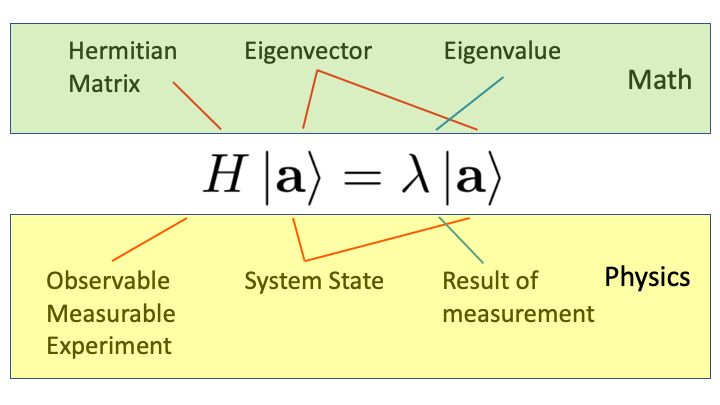
\includegraphics[scale=0.35, frame] {images/math_physics.png}}
\caption{Mathematical and physical interpretation of $H \ket{a} = \lambda \ket{a}$}
\label{fig:math_physics}
\end{figure}


\bigskip
\noindent
Looking ahead, the Hermitian matrix (operator) $H$ will represent something that is \emph{observable} or \emph{measurable}, i.e.,  an \emph{experiment}, 
the eigenvector $\ket{a}$ represents the \emph{state} of the system and the eigenvalue $\lambda \in \mathbb{R}$ represents the actual outcome of the 
measurements. This is illustrated (I hope) in Figure \ref{fig:math_physics}.

\subsection{Review: Orthonormality, Completeness, and Projection}
As we saw above, unitary matrices are matrices which satisfy 

\begin{equation}
\mathbf{U}^{-1} = \mathbf{U}^{\dagger}
\label{eqn:inverse}
\end{equation}

\bigskip
\noindent
Unitary matricies are ubiquitous and important in quantum mechanics, in 
particular because they have the following unique and useful properties: Orthonormality, Completeness, and Projection. We'll briefly look at each of these below\footnote{I will use the 
notation $\begin{pmatrix} x_1, \hdots, x_n \end{pmatrix}^{\text{T}}$ and $\begin{bmatrix} x_1, \hdots, x_n \end{bmatrix}^\text{T}$ interchangably in the following discussion.}.

\subsubsection{Orthornomality}
We can rewrite Equation \ref{eqn:inverse} as

\begin{equation}
\mathbf{U}^{\dagger} \mathbf{U} = \mathbf{I}
\label{eqn:dagger}
\end{equation}

\bigskip
\noindent
where \textbf{I} is the identity matrix. What Equation \ref{eqn:dagger} is really telling us is that the columns of the matrix \textbf{U} form a set of orthnormal vectors.

\bigskip
\noindent
Note that we can interpret a matrix as a row vector where the entries are the columns  $\mathbf{v}_i$ of \textbf{U}. That is

\begin{equation*}
\mathbf{U} = \begin{bmatrix} \mathbf{v}_1 & \mathbf{v}_2 & \hdots & \mathbf{v}_{N} \end{bmatrix}
\end{equation*}

\bigskip
\noindent
Similarly, $\mathbf{U}^{-1}$ can be written as a column vector where the entries are the row vectors $ \mathbf{v}_{i}^\dagger$:

\begin{equation*}
\mathbf{U}^{-1} = \mathbf{U}^{\dagger} = \begin{bmatrix} \mathbf{v}_1^\dagger \\ \mathbf{v}_2^\dagger \\ \vdots  \\ \mathbf{v}_{N}^\dagger  \end{bmatrix}
\end{equation*}

\bigskip
\noindent
Now we can see that 

\begin{flalign*}
\mathbf{U}^{\dagger} \mathbf{U} &= \begin{bmatrix} \mathbf{v}_1^\dagger \\ \mathbf{v}_2^\dagger \\ \vdots  \\ \mathbf{v}_{N}^\dagger  \end{bmatrix}
 \begin{bmatrix} \mathbf{v}_1 & \mathbf{v}_2 & \hdots & \mathbf{v}_{N} \end{bmatrix}  \\
 &= 
 \begin{bmatrix}  
 \mathbf{v}_1^\dagger  \cdot  \mathbf{v}_1 & \mathbf{v}_1^\dagger  \cdot  \mathbf{v}_2 &  \mathbf{v}_1^\dagger  \cdot  \mathbf{v}_3 & \hdots & \mathbf{v}_1^\dagger  \cdot  \mathbf{v}_N \\
 \mathbf{v}_2^\dagger  \cdot  \mathbf{v}_1 & \mathbf{v}_2^\dagger  \cdot  \mathbf{v}_2 &  \mathbf{v}_2^\dagger  \cdot  \mathbf{v}_3 & \hdots & \mathbf{v}_2^\dagger  \cdot  \mathbf{v}_N \\
 \mathbf{v}_3^\dagger  \cdot  \mathbf{v}_1 & \mathbf{v}_3^\dagger  \cdot  \mathbf{v}_2 &  \mathbf{v}_3^\dagger  \cdot  \mathbf{v}_3 & \hdots & \mathbf{v}_3^\dagger  \cdot  \mathbf{v}_N \\
 \vdots & \vdots & \vdots &\ddots & \vdots \\
 \mathbf{v}_N^\dagger  \cdot  \mathbf{v}_1 & \mathbf{v}_N^\dagger  \cdot  \mathbf{v}_2 &  \mathbf{v}_N^\dagger  \cdot  \mathbf{v}_3 & \hdots & \mathbf{v}_N^\dagger  \cdot  \mathbf{v}_N 
 \end{bmatrix} \\
 &= \mathbf{I}
\end{flalign*}

\bigskip
\noindent
or in Dirac notation

\begin{flalign*}
\mathbf{U}^{\dagger} \mathbf{U} &= \begin{bmatrix} \mathbf{v}_1^\dagger \\ \mathbf{v}_2^\dagger \\ \vdots  \\ \mathbf{v}_{N}^\dagger  \end{bmatrix}
 \begin{bmatrix} \mathbf{v}_1 & \mathbf{v}_2 & \hdots & \mathbf{v}_{N} \end{bmatrix} \\
 &= 
 \begin{bmatrix} 
 \bra{v_1} \\  \bra{v_2} \\ \vdots \\ \bra{v_N} 
\end{bmatrix}
 \begin{bmatrix} 
 \ket{v_1} &  \ket{v_2} & \hdots & \ket{v_N} 
\end{bmatrix} \\
&= 
\begin{bmatrix}  
\braket{v_1 | v_1} & \braket{v_1 | v_2} & \braket{v_1 | v_3} & \hdots & \braket{v_1 | v_N} \\
\braket{v_2 | v_1} & \braket{v_2 | v_2} & \braket{v_2 | v_3} & \hdots & \braket{v_2 | v_N} \\
\braket{v_3 | v_1} & \braket{v_3 | v_2} & \braket{v_3 | v_3} & \hdots & \braket{v_3 | v_N} \\
\vdots & \vdots & \vdots & \ddots &   \vdots \\
\braket{v_N | v_1} & \braket{v_N | v_2} & \braket{v_N | v_3} & \hdots & \braket{v_N | v_N} 
\end{bmatrix}  \\
&= \mathbf{I}
\end{flalign*}

\bigskip
\noindent
What we can notice\footnote{$\delta_{ij}$ is the Kronecker Delta function \cite{wiki:kronecker_delta}, $\delta_{ij} = \bigg \{
\begin{array}{ll}
1 & {\rm when  ~}  i = j \\
0 & {\rm when  ~}  i \ne j 
\end{array}$}
here is that since $(\mathbf{U}^{\dagger} \mathbf{U})_{ij} = (\mathbf{U}^{-1} \mathbf{U})_{ij} = \delta_{ij}$,  
the columns of \textbf{U} can be written as the inner product  $\braket{v_i | v_j} = \delta_{ij}$. Said another way,
the vectors $v_i$ form an orthonormal set. In particular, if $\mathbf{V} = \{v_j\}$ is an orthonormal set, then for  $v_i, v_j \in \mathbf{V}$,
the inner product $\braket{v_i | v_j} = \delta_{ij}$.

\subsubsection{Completeness}
From $\mathbf{U}^\dagger \mathbf{U} = \mathbf{I}$ we saw that we could derive orthonormality. But we also expect that $\mathbf{U} \mathbf{U}^\dagger = \mathbf{I}$.
It turns out that we can get something interesting by observing this. In particular 

\begin{flalign*}
\mathbf{U} \mathbf{U}^\dagger &= \begin{bmatrix} \ket{v_1} &  \ket{v_2} & \ket{v_3} & \hdots & \ket{v_N} \end{bmatrix} 
\begin{bmatrix} \bra{v_1} \\ \bra{v_2} \\ \bra{v_3} \\ \vdots \\ \bra{v_N} \end{bmatrix} = \mathbf{I}
\end{flalign*}

\bigskip
\noindent
If we multiply this out, we find that

\begin{equation}
\ket{v_1}\bra{v_1} + \ket{v_2} \bra{v_2} + \cdots + \ket{v_N} \bra{v_N} = \sum\limits_{i = 1}^{N} \ket{v_i} \bra{v_i} = \mathbf{I}
\label{eqn:completeness}
\end{equation}

\bigskip
\noindent
Equation \ref{eqn:completeness} is known as the \emph{completeness} relation. Completeness turns out to be useful and is a sort of
flip-side of orthonormality. While orthonormality is kind of an "inner product" ($\mathbf{U}^{\dagger}\mathbf{U}$), completeness is 
like an outer product in that $\mathbf{U}\mathbf{U}^\dagger$ is a sum over $i$ of $\ket{v_i}\bra{v_i}$. Interestingly, the trace of the outer product of two 
$n \times 1$ column vectors \textbf{a} and \textbf{b} is $\text{Tr}(\ket{a}\bra{b}) = \braket{a | b}$.

\subsubsection{Projection}
To get an idea of what projection is all about, consider the expansion of a vector into components in a basis:

\begin{equation}
\ket{w} =  \sum\limits_{i = 1}^{N} w_i \ket{v_i}
\label{eqn:ket_w}
\end{equation}

\bigskip
\noindent
Now, if the set of vectors basis vectors  $\{v_i\}$ are orthonormal, then we know that 

\begin{equation*}
w_i  =  \braket{v_i  | w}
\end{equation*}

\bigskip
\noindent
and substituting back into Equation \ref{eqn:ket_w} we get

\begin{equation*}
\ket{w} =  \sum\limits_{i = 1}^{N}  \braket{v_i  | w} \ket{v_i}
\end{equation*}

\bigskip
\noindent
Interestingly, there is another way to derive this result:  use the completeness relation, which is simply a fancy but useful way to write \textbf{I}:

\begin{equation*}
\ket{w} =  \mathbf{I} \cdot \ket{w} =  \Bigg (\sum\limits_{i = 1}^{N}  \ket{v_i} \bra{v_i} \Bigg ) \ket{w} = \sum\limits_{i = 1}^{N}  \ket{v_i} \braket{v_i | w}
\end{equation*} 

\bigskip
\noindent
In words, we were able to use the completeness relation to project a vector onto its components in a particular basis.

\bigskip
\noindent
For example, we know that for vectors $\ket{\alpha}$ and $\ket{\beta}$, we can take the inner product between them by using their components in a basis $\{v_i\}$:

\bigskip
\begin{equation*}
\braket{\alpha  | \beta} = \sum\limits_{i = 1}^{N} a_i^* b_i
\end{equation*} 

\bigskip
\noindent
where $a_i = \braket{v_i | \alpha}$ and $b_i = \braket{v_i | \beta}$. Interestingly, we can again derive this using the completeness relation:

\begin{flalign*}
\braket{\alpha | \beta} &= \bra{\alpha}  \mathbf{I} \ket{\beta} 
\: \qquad\qquad \qquad \qquad \qquad \mathrel{\#} \braket{\alpha | \beta} = \bra{\alpha} \ket{\beta} = \bra{\alpha}  \mathbf{I} \ket{\beta} \\
&= \bra{\alpha} \Bigg (\sum\limits_{i = 1}^{N}  \ket{v_i} \bra{v_i} \Bigg )  \ket{\beta} 
 \qquad\qquad \mathrel{\#} \sum\limits_{i = 1}^{N}  \ket{v_i} \bra{v_i}   = \mathbf{I}  \;\; (\text{Equation } \ref{eqn:completeness}) \\
&= \sum\limits_{i = 1}^{N} \braket{\alpha | v_i} \braket{v_i | \beta} 
  \quad \qquad\qquad\qquad \mathrel{\#}  \text{rearrange} \\
&= \sum\limits_{i = 1}^{N} \braket{v_i | \alpha}^* \braket{v_i | \beta} 
\; \;  \qquad \qquad\qquad \mathrel{\#} \braket{a | b} = \braket{ b | a}^* \text{so} \braket{\alpha | v_i}  = \braket{v_i | \alpha}^* \\
&=  \sum\limits_{i = 1}^{N} a_i^*b_i
\; \;  \qquad \qquad\qquad\qquad\qquad \mathrel{\#} a_i^* =  \braket{v_i | \alpha}^*  \text{ and } b_i = \braket{v_i | \beta}
\end{flalign*}

\newpage

\subsection{Photon Polarization Examples}

We know from experimental evidence that ... TBD

\begin{figure}[H]
\center{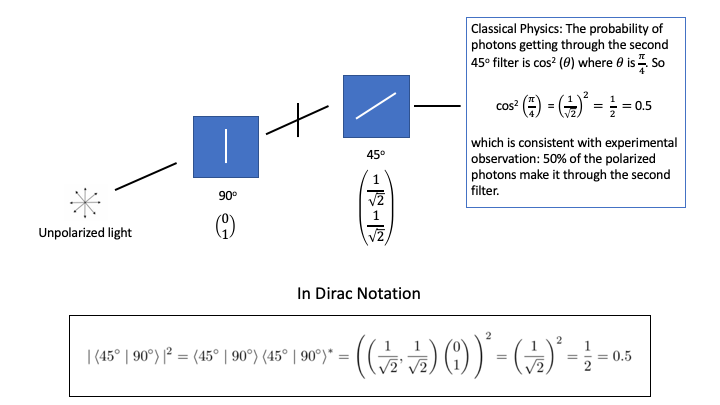
\includegraphics[scale=0.35] {images/90-45.png}}
\caption{\footnotesize What is the probability of a vertically polarized photon getting through a $\ang{45}$ polarizer?}
\label{fig:90-45}
\end{figure}


\begin{equation*}
|\braket{\ang{45} \mid \ang{90}}|^2 = 
\braket{\ang{45} \mid \ang{90}} \braket{\ang{45} \mid \ang{90}}^*
=
\Bigg ( \bigg ( \frac{1}{\sqrt{2}},  \frac{1}{\sqrt{2}} \bigg ) 
\begin{pmatrix}
0\\
1
\end{pmatrix}
\Bigg )^2  =
\bigg ( \frac{1}{\sqrt{2}} \bigg )^2 = \frac{1}{2} = 0.5
\end{equation*}

\bigskip
\noindent
Here 

\begin{equation*}
\ket{\theta} =
\begin{pmatrix}
\alpha \\
\beta
\end{pmatrix}
= \alpha \ket{x} + \beta \ket{y}
\end{equation*}

\noindent
where 

\begin{flalign*}
\alpha &= \cos(\theta) \\
\beta &= \sin(\theta)
\end{flalign*}

\bigskip
\noindent
and the \emph{basis vectors}  $\ket{x}$ and $\ket{y}$ are

\begin{flalign*}
\ket{x} &= \begin{pmatrix}
\cos(0) \\
\sin(0) \\
\end{pmatrix} 
= \begin{pmatrix}
1 \\
0 \\
\end{pmatrix} \\
\ket{y} &= 
\begin{pmatrix}
\cos(\frac{\pi}{2}) \\
\sin(\frac{\pi}{2})  \\
\end{pmatrix} 
=
\begin{pmatrix}
0 \\
1 
\end{pmatrix}
\end{flalign*}

\bigskip
\noindent
These basis vectors can be thought of as a vector
$\begin{pmatrix}
x\\
y
\end{pmatrix}$
\bigskip
\noindent
where $x$ is the projection of a vector $r$ on to the $x$ axis and $y$ is the projection of $r$ on the $y$ axis. This is depicted in Figure \ref{fig:theta}.
\bigskip


\begin{figure}[H]
\center{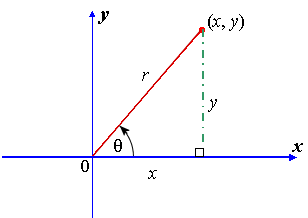
\includegraphics[scale=0.65] {images/theta.png}}
\caption{Two Dimensional Space}
\label{fig:theta}
\end{figure}


\bigskip
\noindent
Back to our example: here the matrix representation of $(\alpha_{0}\ket{0} +\alpha_{1}\ket{1}) + (\beta_{0}\ket{0} +\beta_{1}\ket{1})$ 
is the tensor product

\begin{flalign*}
\begin{pmatrix}
\alpha_0\\
\alpha_1
\end{pmatrix}
\otimes
\begin{pmatrix}
\beta_0\\
\beta_1
\end{pmatrix}
=
\begin{pmatrix}
\alpha_{0} \beta_0 \\
\alpha_{0} \beta_1 \\
\alpha_{1} \beta_0 \\
\alpha_{1} \beta_1 
\end{pmatrix}
\end{flalign*}

\bigskip
\subsection{The \emph{Hadamard} Transform}
As mentioned above, a unitary matrix that acts on a small number of qubits is often called a gate, in analogy to classical logic gates like AND, OR, and NOT. Two simple but important 1-qubit gates are the bit-flip gate X (which negates the bit, i.e., swaps $\ket{0}$ and $\ket{1}$) and the phase-flip gate Z (which puts a $-$ in front of $\ket{1}$). The $2 \times 2$ unitary matrix representations of $X$ and  $Z$ are

\begin{flalign*}
X = 
\begin{pmatrix}
0 & 1\\
1 & 0
\end{pmatrix}
\textrm{,} \;\;
Z = 
\begin{pmatrix}
1 & 0 \\
0 & -1
\end{pmatrix}
\end{flalign*}

\bigskip
\noindent
Another important 1-qubit gate is the \emph{phase gate} $R_{\phi}$, which rotates the phase of the $\ket{1}$-state by an angle $\phi$ such that
\begin{flalign*}
R_{\phi}\ket{0} &= \ket{0} \\
R_{\phi}\ket{1} &= e^{i\phi}\ket{1}
\end{flalign*}
\bigskip
\noindent
This corresponds to the unitary matrix

\begin{flalign*}
R_{\phi} = 
\begin{pmatrix}
1 & 0\\
0 & e^{i\phi}
\end{pmatrix}
\end{flalign*}

\bigskip
\noindent
Interestingly $Z$ is a special case of $R_{\phi}$: $Z = R_{\pi}$ since by Euler's identity $e^{i\pi} =  -1$.

\bigskip
\noindent
Possibly the most important 1-qubit gate is the \emph{Hadamard transform},  specified by:

\begin{flalign*}
H \ket{0} &= \frac{1}{\sqrt{2}}\ket{0} + \frac{1}{\sqrt{2}}\ket{1}\\
H\ket{1} &= \frac{1}{\sqrt{2}}\ket{0}  - \frac{1}{\sqrt{2}}\ket{1}
\end{flalign*}

\bigskip
\noindent
The  (unitary) matrix representation of \emph{Hadamard transform} is then
\begin{flalign*}
H = \frac{1}{\sqrt{2}}
\begin{pmatrix}
1 & 1\\
0 & -1
\end{pmatrix}
\end{flalign*}

\bigskip
\noindent
If we apply $H$ to initial state $\ket{0}$ and then measure, we have equal probability of observing $\ket{0}$
or $\ket{1}$. Similarly, applying $H$ to $\ket{1}$ and observing gives equal probability of $\ket{0}$  or $\ket{1}$. 

\bigskip
\noindent
However, if we apply $H$ to the superposition $\frac{1}{\sqrt{2}}\ket{0} + \frac{1}{\sqrt{2}}\ket{1}$ we get $\ket{0}$, since

\begin{flalign*}
H \ket{0} &= \frac{1}{\sqrt{2}}\ket{0} + \frac{1}{\sqrt{2}}\ket{1} \\
H \ket{1} &= \frac{1}{\sqrt{2}}\ket{0} - \frac{1}{\sqrt{2}}\ket{1} \\
H( \frac{1}{\sqrt{2}}\ket{0} + \frac{1}{\sqrt{2}} \ket{1}) &= \frac{1}{2}(\ket{0}) + \ket{1}) + \frac{1}{2}(\ket{0}) - \ket{1}) 
= \ket{0} \\
H( \frac{1}{\sqrt{2}}\ket{0} - \frac{1}{\sqrt{2}} \ket{1}) &= \frac{1}{2}(\ket{0}) + \ket{1}) - \frac{1}{2}(\ket{0}) - \ket{1}) 
= \ket{1}
\end{flalign*}

\bigskip
\noindent
What has happened here is that the positive and negative amplitudes for $\ket{1}$ have canceled out\footnote{This also means that $H$ is its own inverse.}. This effect is called \emph{interference}, and is analogous to interference patterns between light or sound waves. We will see this again in Section \ref{sec:exp}.

\bigskip
\noindent
Finally, notice that one application of the Hadamard gate to either a 0 or 1 qubit will produce a quantum state that, if observed, will be a 0 or 1 with equal probability. This is exactly like flipping a fair coin in the standard probabilistic model of computation. However, if the Hadamard gate is applied twice in succession, then the final state is always the same as the initial state. This would be like taking a fair coin that is showing heads, flipping it twice, and it always landing on heads after the second flip.

\bigskip
\subsection{One More Example: CNOT}
We can also represent gates acting on more than one wire. For example, consider the controlled-not gate, denoted CNOT. This is a gate that acts on two bits, labelled the control bit ($c$) and the target bit ($t$). The action of the 
gate is to apply the not operation to the target if the control bit is 0, and do nothing otherwise (the control bit is always unaffected by the CNOT gate). Equivalently, if the state of the control bit is $c$, and the target bit is in state t the CNOT gate maps the target bit to $t \oplus c$ (where $\oplus$  represents the logical exclusive-or operation, or addition modulo 2). The CNOT gate is illustrated in Figure  \ref{fig:cnot}.



\begin{figure}[H]
\center{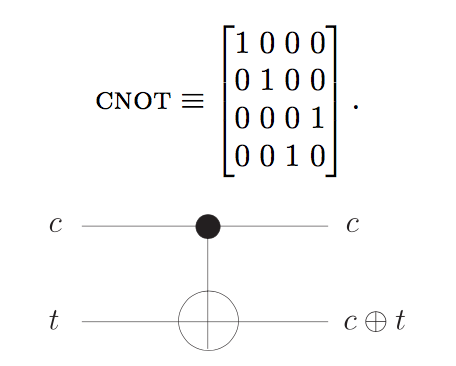
\includegraphics[scale=0.8] {images/cnot.png}}
\caption{The \emph{reversible} CNOT gate flips the value of the $t$ iff the control bit $c = 1$ }
\label{fig:cnot}
\end{figure}

\bigskip
\noindent
Consider a pair of wires such that the first wire is in state 1 and the second in state 0. This means that the 4-dimensional vector describing the combined state of the pair of wires is

\begin{flalign}
\begin{pmatrix}
0\\
0 \\
1 \\
0
\end{pmatrix}
\label{eqn:bits}
\end{flalign}

\bigskip
\noindent
We now  want to apply the CNOT gate to a pair of wires shown in Equation \ref{eqn:bits} where we interpret the first wire as the control bit and the second as the target bit. From the description of the CNOT gate, we expect the result should be that the control bit (first wire) remains in state 1, and the target bit (second wire) flips to state 1. That is, we expect the resulting state vector to be

\begin{flalign*}
\begin{pmatrix}
0\\
0 \\
0 \\
1
\end{pmatrix}
\end{flalign*}

\noindent
That is
\begin{flalign*}
\text{CNOT}
\begin{pmatrix}
0\\
0 \\
1 \\
0
\end{pmatrix}
\equiv
\begin{pmatrix}
1 & 0 & 0 & 0 \\
0 & 1 & 0 & 0 \\
0 & 0 & 0 & 1 \\
0 & 0 & 1 & 0
\end{pmatrix}
\begin{pmatrix}
0\\
0 \\
1 \\
0
\end{pmatrix}
=
\begin{pmatrix}
0\\
0 \\
0 \\
1
\end{pmatrix}
\end{flalign*}


\section{Beam Splitters}
Suppose we have an experimental setup consisting of a photon source, a beam splitter (which was once implemented using a half-silvered mirror), and a pair of photon detectors. This is the classic beam splitter setup, and is illustrated in Figure \ref{fig:one_beam_splitter_setup}.

\bigskip
\noindent
Suppose we send a series of individual photons along a path from the photon source towards the beam splitter. We observe the photon arriving at the detector on the right on the beam splitter half of the time, and arriving at the detector above the beam splitter half of the time, as illustrated in Figure \ref{fig:measurement_statistics_with_one_beam_splitter}. Perhaps the simplest way to explain this behavior in a theory of physics is to model the beam splitter as effectively flipping a fair coin, and choosing whether to transmit or reflect the
photon based on the result of the coin-flip, whose outcome determines whether the photon is transmitted or reflected.
This is very similar to the behavior of a probabilistic Turing machine. 


\begin{figure}
\center{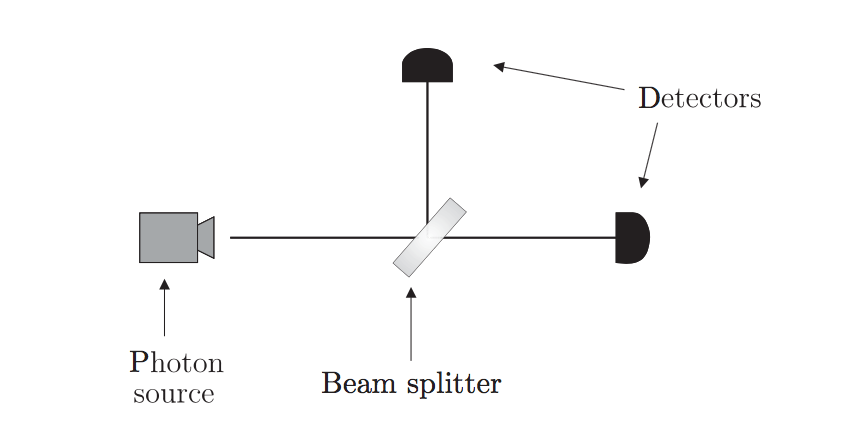
\includegraphics[scale=0.8] {images/one_beam_splitter_setup.png}}
\caption{Experimental setup with one beam splitter}
\label{fig:one_beam_splitter_setup}
\end{figure}



\bigskip
\noindent
Now consider a modification of the setup shown in Figure \ref{fig:one_beam_splitter_setup}
with  a pair of beam splitters and fully reflecting mirrors to direct the photons along either of two paths as shown in Figure \ref{fig:2_beam_splitters}, where the paths are labelled 0 and 1. This setup is the
famous  the Mach-Zehnder interferometer \cite{0031-9120-35-1-308}  It is important to note that the length of paths 0 and 1 are equal, so the photons arrive at the same time, regardless of which path is taken.

\bigskip
\noindent
By treating the beam splitters as independently deciding at random whether to transmit or reflect incident photons, classical physics predicts that each of the detectors will register photons arriving 50 per cent of the time, on average. Here, however, the results of experiments reveal an entirely different behavior. However, what we find is that the photons arrive at only one of the detectors, 100 per cent of the time. This is shown in Figure \ref{fig:measurement_statistics_with_two_beam_splitters}. But why?


\bigskip
\noindent
The result of the  experiment  shown in Figure  \ref{fig:measurement_statistics_with_two_beam_splitters} is at the very least counter-intuitive, largely because it does not agree with our classical intuition. However, quantum physics models the experiment in a way that correctly predicts the observed outcomes. The non-intuitive behavior results from features of quantum mechanics called \emph{superposition} and \emph{interference}. Let's take a look at a framework that can  explain the results of this experiment.

\bigskip
\noindent
First, let's suppose that the second beam splitter were not present in the apparatus. Then the photon follows one of two paths (according to classical physics), depending on whether it is reflected or transmitted by the first beam splitter. If it is transmitted through the first beam splitter, the photon arrives at the top detector, and if it is reflected, the photon arrives at the detector on the right. We can consider a photon in the apparatus as a 2-state system, letting the presence of the photon in one path represent a 0 and letting the presence of the photon in the other path represent a 1.

\begin{figure}
\center{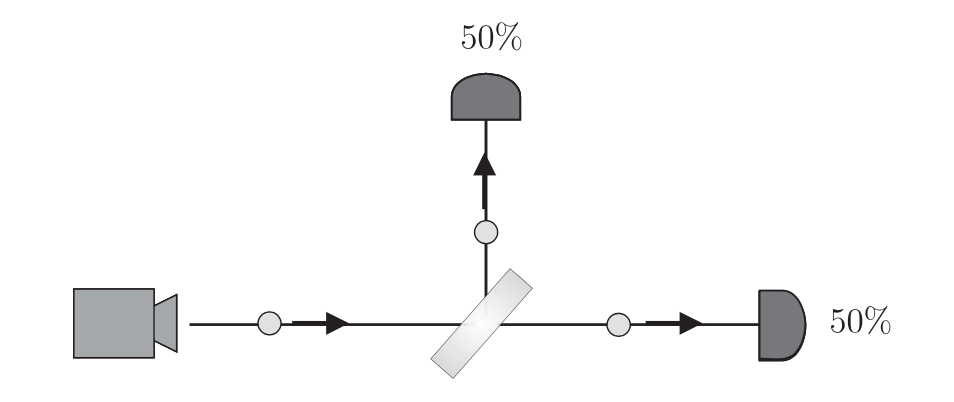
\includegraphics[scale=0.8] {images/measurement_statistics_with_one_beam_splitter.png}}
\caption{Experimental setup with one beam splitter}
\label{fig:measurement_statistics_with_one_beam_splitter}
\end{figure}

\bigskip
\noindent
Following our approach with classical circuits, we denote the state of a photon in path 0 by the vector
\begin{flalign*}
\begin{pmatrix}
1 \\
0
\end{pmatrix}
\end{flalign*}

\bigskip
\noindent
and a photon in path 1 by the vector 
\begin{flalign*}
\begin{pmatrix}
0\\
1
\end{pmatrix}
\end{flalign*}

\bigskip
\noindent
By convention, the photon leaving the source starts out in the 0 path. In a classical description, we model the beam splitter as randomly selecting whether the photon will continue along the 0 path, or be reflected into the 1 path. According to the quantum mechanical description, the beam splitter causes the photon to go into a superposition of taking both the 0 and 1 paths. Mathematically, we describe such a superposition by taking a linear combination of the state vectors for the 0 and 1 paths, so the general path state will be described by the vector shown in Equation \ref{eqn:alphas}.

\bigskip
\noindent
If we were to physically measure the photon to see which path it is in, we will find it in path 0 with probability 
$|\alpha_0|^2$ and in path 1 with probability $|\alpha_1|^2$.  Measuring a superposition\footnote{Quantum mechanics requires that the superposition of states be a linear combination.} $\ket{\phi} = \alpha_{0}\ket{0} + \alpha_{1}\ket{1} + \cdots + \alpha_{j}\ket{j} + \cdots + \alpha_{n}\ket{n-1}$ collapses it into an observed state $\ket{j}$, where  the probability of observing state $\ket{j}$ is $|\alpha_{j}|^2$. Thus\footnote{Note that the absolute square of a complex number $z$,  $|z|^2$, is defined to as follows:  $|z|^2 = z \bar{z}$ where $\bar{z}$ denotes the \emph{complex conjugate} of $z$ and $|z|$ is the \emph{complex modulus}.}

\begin{equation*}
\sum\limits_{i = 0}^{n-1} |\alpha_{i}|^2 = 1
\end{equation*}
That is, if we measure $\ket{\phi}$ we will observe the n-bit state state $\ket{j}$ with probability $|\alpha_{j}|^2$. In our example, $|\alpha_0|^2 + |\alpha_1|^2 = 1$ and

\begin{equation*}
\alpha_{0} 
\begin{pmatrix}
1\\
0
\end{pmatrix}
+
\alpha_1 
\begin{pmatrix}
0\\
1
\end{pmatrix}
=
\begin{pmatrix}
\alpha_0\\
\alpha_1
\end{pmatrix}
\label{eqn:alphas}
\end{equation*}


\begin{figure}
\center{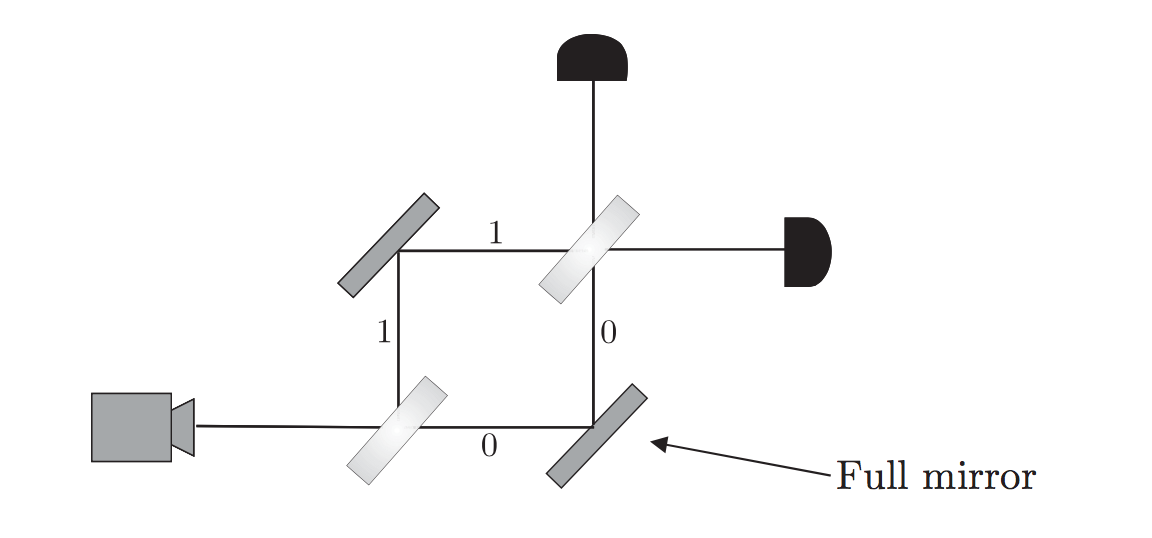
\includegraphics[scale=0.8] {images/2_beam_splitters.png}}
\caption{Experimental setup with two beam splitters: the Mach-Zehnder interferometer}
\label{fig:2_beam_splitters}
\end{figure}

\subsection{A Little More on Superposition}

Consider some physical system that can be in N different, mutually exclusive classical states. Call these states 
$\ket{0}, \ket{2}, \cdots,  \ket{N-1}$. A \emph{classical state} is a state in which the system can be found if we observe it (with some details). A \emph{pure quantum state} (usually just called state) $\ket{\phi}$ is a superposition of classical states, written\footnote{$\ket{i}$ is the \emph{ket} part of the Dirac \emph{bra-ket} notation.}
\begin{flalign*}
\ket{\phi} = \alpha_0 \ket{0} + \alpha_2 \ket{2} + \cdots + \alpha_{N-1} \ket{N-1}
\end{flalign*}

\noindent
Here $\alpha_i$ is a complex number called the \emph{amplitude} of $\ket{i}$. Intuitively, a system in quantum state
$\ket{\phi}$ is in all classical states at the same time (!). In particular,  it is in state $\ket{0}$ with amplitude $\alpha_0$, in state $\ket{1}$ with amplitude $\alpha_1$, and so on. Mathematically, the states 
$\ket{0}, \cdots, \ket{N-1}$ form an orthonormal basis of an N-dimensional Hilbert space (i.e., an N-dimensional vector space equipped with an inner product) of dimension N, and a quantum state $\ket{\phi}$ is a vector in this space.

\subsection{Quantum Memory}
In classical computation, the unit of information is a bit, which can be 0 or 1. In quantum computation, this unit is a quantum bit (\emph{qubit}), which is a superposition of 0 and 1. Consider a system with 2 basis states, call them $\ket{0}$ and $\ket{1}$. We identify these basis states with the vectors  $\begin{pmatrix} 1\\ 0 \end{pmatrix}$ and $\begin{pmatrix} 0\\ 1 \end{pmatrix}$ respectively. As mentioned above,  a single qubit can be in any superposition
$\ket{\phi} = \alpha_{0} \ket{0} + \alpha_{1} \ket{1}$ with 
$|\alpha_{0}|^2 + |\alpha_{1}|^2 = 1$. This latter condition is sometimes called the \emph{normalization constraint}. Again, $|\alpha_{0}|^2$ is the probability of finding the qubit in state $\ket{0}$. Similarly,  $|\alpha_{1}|^2$ is the probability of finding the qubit in state $\ket{1}$. 

\bigskip
\noindent
Finally, it is worth noting that a complex amplitude $\alpha$ can be decomposed into the (unique) product $e^{i\theta}|\alpha|$, where $|\alpha|$ is the non-negative real number corresponding to the magnitude of $\alpha$, and $e^{i\theta} = \frac{\alpha}{|\alpha|}$ has norm 1. $\theta$ is known as the phase and $e^{i\theta}$ is the phase factor.
What is important about this is that the state vector described by $e^{i\theta}\ket{\psi}$ is equivalent to the state vector described by $\ket{\psi}$ where $e^{i\theta}$ is any complex vector with unit norm. For example, the state
$\ket{0} + \ket{1}$ is equivalent to the state vector described by $e^{i\theta}\ket{0} + e^{i\theta}\ket{1}$.

\bigskip
\noindent
A single qubit "lives" in the vector space $\mathbb{C}^2$.  Systems of more than 1 qubit "live"  in the tensor product space of several qubit systems. For example, a 2-qubit system has 4 basis states: $\ket{0} \otimes \ket{0}$,  $\ket{0} \otimes \ket{1}$, 
$\ket{1} \otimes \ket{0}$, and $\ket{1} \otimes \ket{1}$. Here $\ket{1} \otimes \ket{0}$ means that the first qubit is in its basis state $\ket{1}$ and the second qubit is in its basis state $\ket{0}$. 

\bigskip
\noindent
More generally, a register of n qubits has $2^n$ basis states, each of the form
\bigskip
\noindent
\begin{flalign}
\ket{b}_0 \otimes \ket{b}_2 \otimes \cdots \otimes \ket{b}_{n-1}\textrm{,} \; 
\textrm {with} \; b_i  \in \{0, 1\}
\end{flalign}

\bigskip
\noindent
We can abbreviate all of this as $\ket{b_0b_2 \cdots b_{n-1}}$. In addition, since bit strings of length $n$ can be viewed as numbers between 0 and $2^n - 1$, we can also write the basis states as 
$\ket{0}, \ket{1}, \ket{2}, \cdots \ket{2^n - 1}$. Thus a quantum register of $n$ qubits can be in any superposition $\phi$ 
\begin{flalign*}
\ket{\phi} = \alpha_{0}\ket{0} + \alpha_{1} \ket{1} + \cdots + \alpha_{2^n - 1}\ket{2^n - 1} \;
\textrm{where}  \;
\sum\limits^{2^n-1}_{j = 0} |a_{j}|^2 = 1
\end{flalign*}


\section{Getting back to the experiment...} 
\label{sec:exp}
Lets call the beam splitter "gate" $M_{BS}$. Then

\begin{flalign*}
\begin{pmatrix}
\alpha_{0}^ \prime\\
\alpha_{1}^\prime
\end{pmatrix}
=
M_{BS}
\begin{pmatrix}
\alpha_{0}\\
\alpha_{1}
\end{pmatrix}
=
\begin{pmatrix}
t_{11} & r_{21} \\
r_{12} & t_{22}
\end{pmatrix}
\begin{pmatrix}
\alpha_{0}\\
\alpha_{1}
\end{pmatrix}
\end{flalign*}

\bigskip
\noindent
where $t_{ij}$  and $r_{ij}$ are the amplitude transmission and reflection factors to and from the different ports of the beam splitter. Rearranging the complex coefficients $t_{ij}$  and $r_{ij}$  yields

\begin{flalign*}
M_{BS} = 
\frac{\exp(i \phi_{0})}{\sqrt{2}}
\begin{pmatrix}
1 & i \\
i & 1 
\end{pmatrix}
\end{flalign*}

\bigskip
\noindent
where $i = \sqrt{-1}$  and $\phi_{0}$ is an arbitrary phase constant usually set to zero. 

\bigskip
\noindent
Hence both of the transmitted light beams undergo a phase-shift of $\frac{\pi}{2}$ while the reflected beams are unaffected.  In summary, when the photon passes through the beam splitter, we multiply its state vector by the splitter matrix

\begin{flalign*}
\frac{1}{\sqrt{2}}
\begin{pmatrix}
1 & i \\
i & 1 
\end{pmatrix}
\end{flalign*}

\bigskip
\noindent
Since we stipulate that the photon starts out in path 0, after passing through the first beam splitter it comes out in state
\begin{flalign*}
\frac{1}{\sqrt{2}}
\begin{pmatrix}
1 & i \\
i & 1 
\end{pmatrix}
\begin{pmatrix}
1 \\
0
\end{pmatrix}
& =
\frac{1}{\sqrt{2}}
\begin{pmatrix}
1 \\
i
\end{pmatrix} \\
&=
\frac{1}{\sqrt{2}}
\begin{pmatrix}
1 \\
0
\end{pmatrix}
+
\frac{i}{\sqrt{2}}
\begin{pmatrix}
0 \\
1
\end{pmatrix}
\end{flalign*}


\begin{figure}
\center{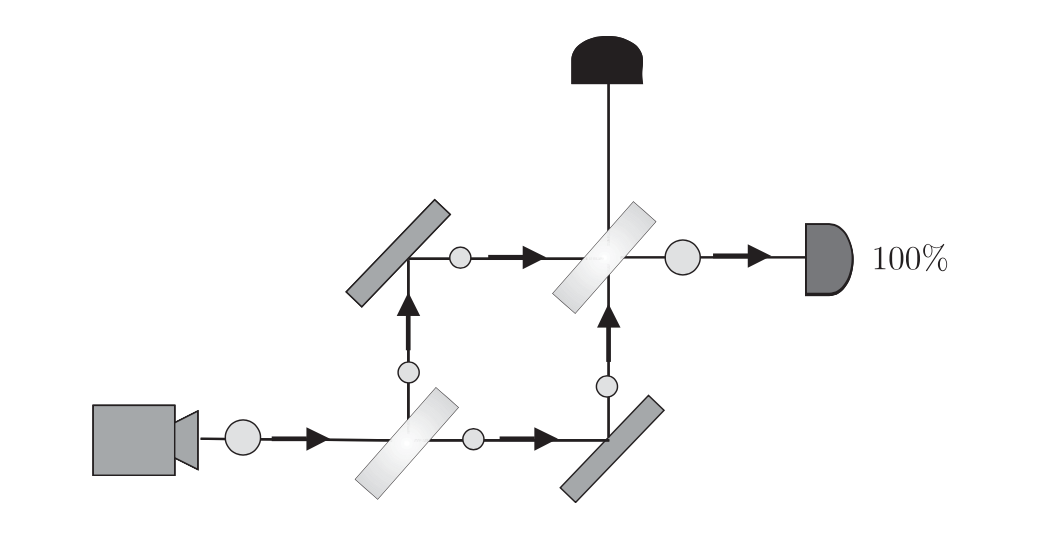
\includegraphics[scale=0.8] {images/measurement_with_two_beam_splitters.png}}
\caption{Experimental setup with two beam splitters}
\label{fig:measurement_statistics_with_two_beam_splitters}
\end{figure}

\bigskip
\noindent
This result corresponds with the observed behavior that after going through the first beam splitter, we would measure the photon in path 0 with probability $|\frac{1}{\sqrt{2}}|^2 = \frac{1}{2}$ and in path 1 with probability $|\frac{i}{\sqrt{2}}|^2 = \frac{1}{2}$.

\bigskip
\noindent
However, if we do not measure which path the photon is in immediately after it passes through the first beam splitter, then its state remains\footnote{Note that 
$\begin{pmatrix}
\alpha_0\\
\alpha_1
\end{pmatrix}$
is alternate notation for 
$\begin{bmatrix}
\alpha_0\\
\alpha_1
\end{bmatrix}$.}

\begin{flalign*}
\frac{1}{\sqrt{2}}
\begin{pmatrix}
1 \\
i
\end{pmatrix}
\end{flalign*}

\bigskip
\noindent
Now (finally getting to the result), if  the photon is allowed to pass through the second beam splitter before making any measurement of the photon's path its new state vector is

\begin{flalign*}
\begin{pmatrix}
\frac{1}{\sqrt{2}}
\begin{pmatrix}
1 & i \\
i & 1 
\end{pmatrix}
\end{pmatrix}
\begin{pmatrix}
\frac{1}{\sqrt{2}}
\begin{pmatrix}
1 \\
i 
\end{pmatrix}
\end{pmatrix}
=
\begin{pmatrix}
0 \\
i 
\end{pmatrix}
\end{flalign*}

\bigskip
\noindent
If we then measure the path of the photon \textbf{after} the second beam splitter (e.g. by the detectors shown in Figure \ref{fig:2_beam_splitters}), we find the photon on 1 path with probability $|i|^2 = 1$ and path 0 with probability $|0|^2 = 0$ (recall that  $|\alpha_0|^2 + \alpha_1|^2 = 1$).  Thus we expect that when we measure the photon after the second beam splitter it will be entirely on path 1, which is what we observe in experiments like the one illustrated in Figure \ref{fig:measurement_statistics_with_two_beam_splitters}. 

\bigskip
\noindent
Finally, the quantum mechanical interpretation of all of this is that the second beam splitter has caused the two paths (that were in \emph{superposition}) to \emph{interfere}, resulting in cancelation of the 0 path.

\section{Acknowledgements}
Marshall Eubanks, Colin Dixion and Chris Wright provided helpful comments on early versions of this document.

\newpage
\bibliographystyle{plain}
\bibliography{/Users/dmm/papers/bib/qc}



\end{document} 
